\documentclass[twocolumn]{article}
\usepackage{graphics}
\usepackage{graphicx}
\usepackage[utf8]{inputenc}
\usepackage{hyperref}
\usepackage{natbib}

\newcommand{\aetitle}{Algorithm Engineering Report 02} % Title of the report
\newcommand{\studentOne}{Patrick Koston} % Name 1
\newcommand{\studentTwo}{Simon Schwitz} % Name 2


\begin{document}

\twocolumn[{\begin{small}
\begin{minipage}{0.5 \linewidth}
  Algorithm Engineering\\
  WS 23/24
\end{minipage}
\begin{minipage}{0.5\linewidth}
  \begin{flushright}
    \studentOne\\
    \studentTwo
  \end{flushright}
\end{minipage}
\end{small}}
{\begin{center}
\begin{sffamily}\Large\bfseries \aetitle \end{sffamily}
\end{center}}
\vskip 3em]

\begin{abstract}
    Abstract is very abstract
\end{abstract}


\section{Introduction}
We like to think about things in sequence. One thought alone, that needs our attention. Else, through distractions, we might lose what we were thinking about or maybe completely lose the thought at hand. But we can multitask, although that is depended on the tasks at hand being different from each other in terms of what section of our brain are targeted.\\
Computers can also multitask, yet instead of having to have thematically different tasks, they can focus all their power on one problem divided, to conquer it faster. That is due to processors and the amount modern computers possess, in contrast to the past, where it was more akin to the first description and needing to use scheduling algorithm, like round-robin scheduling, to simulate parallel work being done on a processor.\\
But to regain focus, in this report we will focus on the parallel implementation of two algorithms, Merge and Quick Sort, and their normal counterparts and how they compare to each other.


\section{Build and Run the project}
%Possibly might do a small rewrite here
In order to build the project you must meet all requirements from the \texttt{README.md} file in the project root directory.
The build script will check whether \texttt{gcc} and \texttt{g++} commands are present on your system. 
Note: it will not check the their version so make sure the required minimum version is installed!\\
\\
In case the build fails, we now also include pre-built binaries in the \texttt{bin/} directory.\\
\\
You can also check the state whether Linux build success or not using the \href{https://gitlab.inf.uni-konstanz.de/ag-storandt/ae-24/koston.schwitz/-/pipelines}{GitlabCI Pipeline}. 
This pipeline uses the latest \texttt{gcc} version which as of writing is \texttt{14.2.0}. 
You can verify this on \href{https://hub.docker.com/_/gcc}{Dockerhub} or when looking into the pipeline result.

\subsection{On Failed Build}
The script then throws an error that the CMake build did fail.
Usually it then still continues with executing the experiments using the pre-build binaries.
In case this should not work, please modify the experiment script using the instructions below:\\
On Windows, please remove lines $8$ and $9$ from the corresponding PowerShell script.\\
On Linux, please remove lines $9$ and $10$ from the corresponding Bash script.

\subsection{Run Experiments}
Working Directory must be the corresponding exercise directory!\\
On Windows, execute the \texttt{experiment\_0\{1,2\}.ps1} scripts in the exercise directory to run the corresponding experiment.\\
On Linux, execute the \texttt{experiment\_0\{1,2\}.sh} scripts in the exercise directory to run the corresponding experiment.\\

\subsection{Source Code / Project Structure}
The source to run the experiments can be found in the \texttt{src/} directory of the current exercise directory. 
Reusable code however is not included in the exercises source directory and can be found in the \texttt{lib/} directory instead. 
To keep the project clean, we reserve to export reusable code to separate libraries which are then linked in the header of the exercise source files. 
Please see the README.md file for information about which shared libraries exist and what they contain.

\section{Preliminaries}
%Theoretical Knowledge applied here
%The algorithm we are wanting to focus on is External Memory MergeSort, or short EM-MergeSort.
%For the task of sorting data entries we are focusing on MergeSort. It functions by firstly dividing all entries into singular entries, then merging them together into parts and sorting them during that process. With this, we can work on smaller arrays of objects.


\section{Algorithm \& Implementation}
%This section provides information about the actually used algorithms and their respective implementations. It should roughly cover the following three topics:
%\begin{itemize}
%	\item \textbf{Advanced Algorithm:}\\
%		Give and explain the advanced algorithms that you used, and compare them to the basic algorithms.
%	\item \textbf{Implementation:}\\
%		Explain how you implemented these algorithms and state what external libraries you used.
%	\item \textbf{Algorithm Engineering Concepts:}\\
%		State the algorithm engineering concepts that you used and explain why they were helpful (if applicable).
%\end{itemize}

\subsection{Implementation}
\subsubsection{Parllell Merge Sort}
The code can be found in \texttt{lib/Sort/mergeSort.cpp} (see included headers).\\
\\
Given a variable $T$ indicating the number of threads to use, the algorithm first checks if the available input data can be split into $T$ buckets of at least $2$ elements. 
If this condition is not met, a classic merge sort will be performed on the data set instead.
In the next step, the input data is partitioned into $T$ buckets of size $input.size()/T$.  
These buckets are then individually sorted using classic merge sort. 
We then apply a similar bottom-up approach to the external memory merge sort and create multiple tasks that each wait for two tasks lower in the tree structure to finish sorting and then performs the merging step on that level. 
During the bottom-up merging, we have $T/2$ tasks at most thus we never exceed the thread limit.
\begin{figure}[h]
    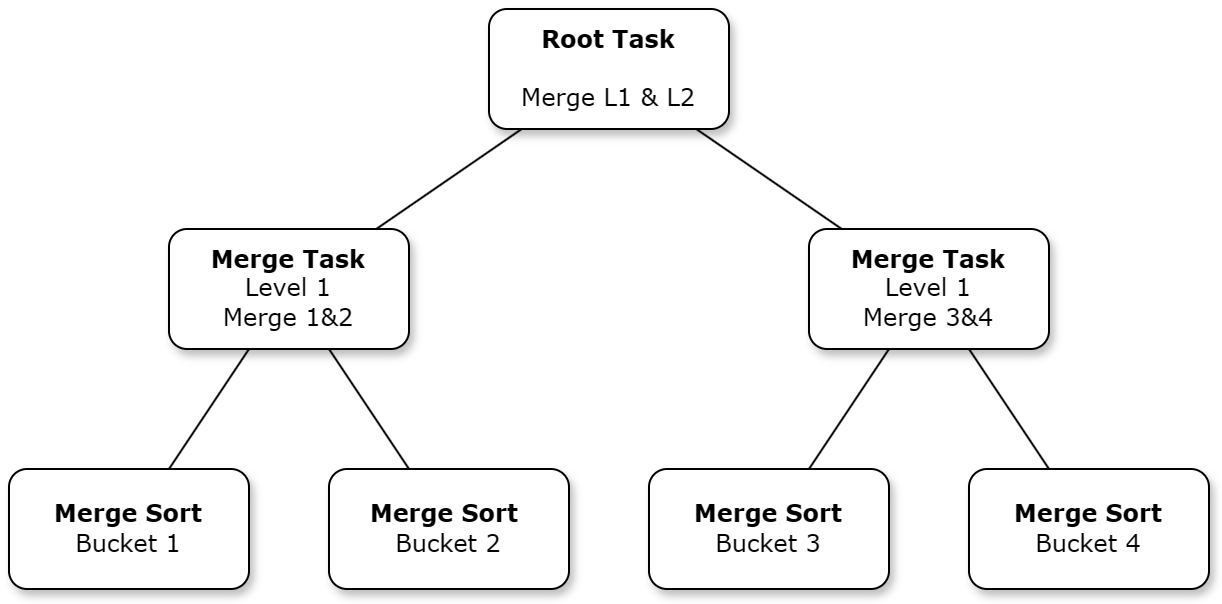
\includegraphics[scale=0.175]{./figures/merge_sort_even.png}
    \centering
    \caption{Parallel merge sort using an even number of $T=4$ buckets}
    \end{figure}
In the event of T being odd, the corresponding merging tasks will wait for a single previous task and then merely pass on the result as there is no second block to merge with. 
Modern computers usually have an even number of cores/threads so we can argue that this case does not occur under normal circumstances.
\begin{figure}[h]
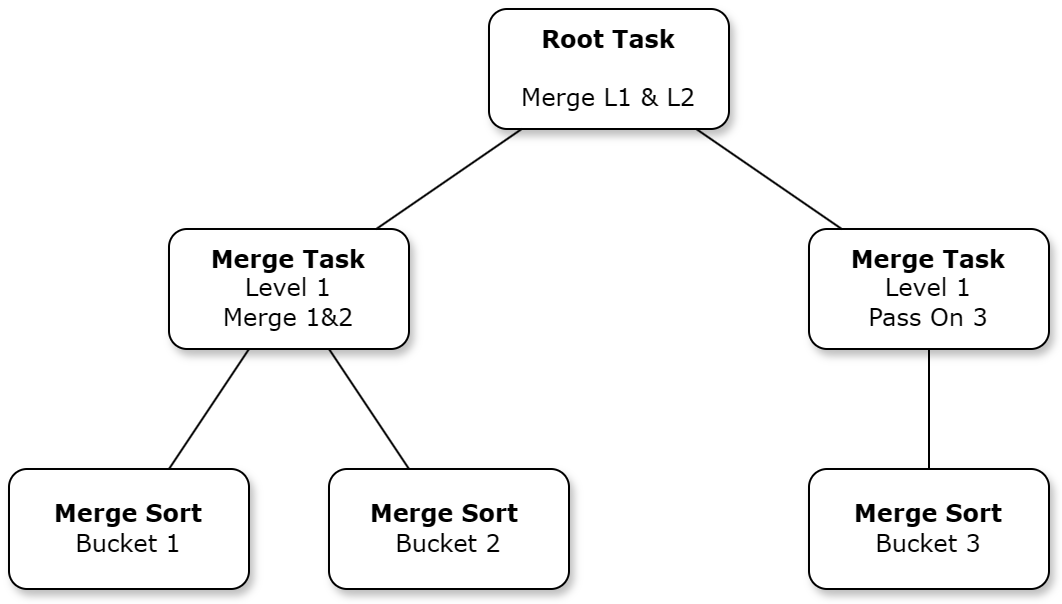
\includegraphics[scale=0.175]{./figures/merge_sort_odd.png}
\centering
\caption{Parallel merge sort using an odd number of $T=3$ buckets}
\end{figure}

\subsubsection{Parallel Quick Sort}
The code can be found in \texttt{lib/Sort/quickSort.cpp} (see included headers).\\ 
\\
Given a variable $T$ indicating the number of threads to use, the algorithm first checks if the available input data can be split into $T$ buckets of at least $2$ elements. 
Additionally, a check is performed if the input size is less than a predefined constant of $1000$. 
In this case, classic merge sort will be performed for performance reasons.\\
If this is not the case we select the number in the middle (rounded down) of the input data as the pivot element. 
In the next step, the input data is partitioned into $T$ buckets of size $input.size()/T$. Each bucket then sorts the data into a left and right half. 
The left half contains only elements smaller than our pivot element and the right side only elements greater than our pivot element. 
To later split the array into a ``smaller than'' and ``larger than'' half, we count the number of elements on each side. 
If the array contains the pivot itself, the pivot is placed in between both halves and is not counted.\\
Once each task has finished splitting, the data is written back into the original array. 
When writing back, we first move all halves smaller than the pivot in the array, then the pivot itself, and then lastly all halves greater than the pivot. 
We also have to keep track of the size of the combined ``smaller than'' and ``greater than'' half. 
In each subsequent step, we then apply the same algorithm to both, the smaller and the greater half. 
We do this until we reach the predefined constant threshold point for input (bucket) size. 
From this point on further branching is way too expensive. 
To reduce runtime costs, the predefined constant should have an even higher value (at least $10,000$).
\begin{figure}[h]
    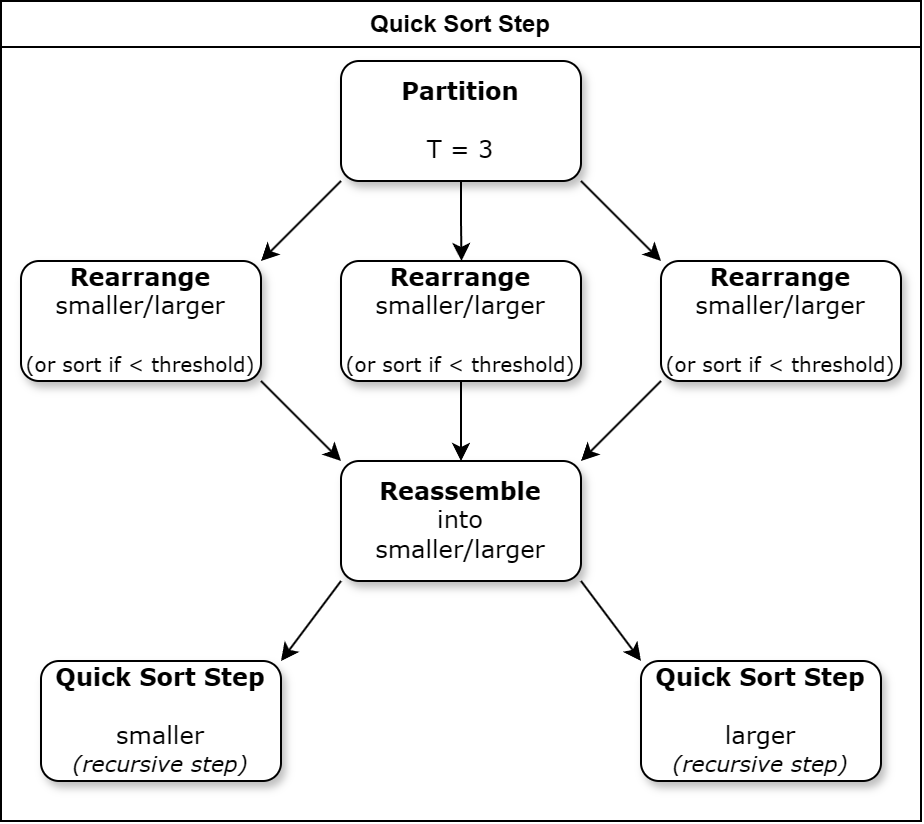
\includegraphics[scale=0.175]{./figures/parallel_quick_sort.png}
    \centering
    \caption{Parallel quick sort using $T=3$ buckets}
\end{figure}

\section{Experimental Evaluation}
The experimental setup for our experiment is described below, along with the findings.

\subsection{Data and Hardware}%
\label{sub:Data and Hardware}
The data used in our experiments are generated by the number generator files \texttt{numberGen} and \texttt{numberGen32}, that can be found in the \texttt{lib/Utils/} directory. This is done to generate a randomized data set according to the definition given in the assignment.\\
The hardware utilized for running this experiment consisted of the following parts. For the CPU, we used an AMD® Ryzen 7 7840HS, which can run 16 Threads. For the RAM unit, we had a size of 32GB available for our runs. The operating system was Zorin OS 17.2, which is based on Ubuntu, namely the 22.04 LTS version.\\
For running the code, we used the 3.22.1 version of cmake and the 13.1.0 version of gcc.


\subsection{Results}%
The results we received from our testing can be viewed in detail in the \texttt{results} directory, namely the files with the suffix \texttt{laptop}.\\
For the first part of our results, we compared the average total time required to finish the sorting, as can be seen in figure~\ref{fig:exp1_totalTime}. Overall, the parallel Merge Sort performed better on all cores compared to the parallel Quick Sort. The minimum for the average time per core for Merge Sort was found at using 15 cores with a time of 24.64430 seconds and the highest using 2 cores with a time of 85.08657 seconds. In stark contrast, the lowest time for Quick Sort was found at 5 cores with a time of 97.96354 seconds and the highest at 2 cores with a time of 121.23832 seconds. Following this, we decided to core amount that resulted in the lowest total time to be viewed as the best possible value $p$ for the second part of the experiment for the parallel Merge Sort and parallel Quick Sort, being 15 and 5 respectively.

\begin{figure}[h]
	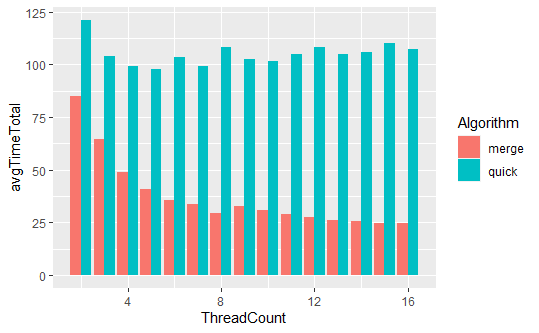
\includegraphics[scale=0.5]{./figures/exp1_comparison_totaltime.png}
	\centering
	\caption{Comparison of average total time per core usage}
	\label{fig:exp1_totalTime}
\end{figure}

For the second part, we focus on the comparison between the type of each algorithm, being single threaded (sta) and multi threaded (mta), as well as the algorithm utilized (Quick Sort, Merge Sort). When comparing them pairwise for each data input size we had, being $10^i$, with $i = 3,...,9$, we were able to see that with a low enough size of i=3, quick sort proved itself faster in both types, as can be seen in figure~\ref{fig:exp2}. But starting with i=4 we can see that the parallel Merge Sort has taken favor in being faster during the sorting. To note, the same applies for the total time, throughout all tests, as it didn't change the comparison from the results we tracked. With i=5 we see an increase in the time required, which will continue drastically with increasing i, but starting here we see a big gap between the time between the parallel Quick Sort and Merge Sort, which stands in opposition to the data collected for their single thread variants. This trend stays consistant through i=9.

\begin{figure}[h]
	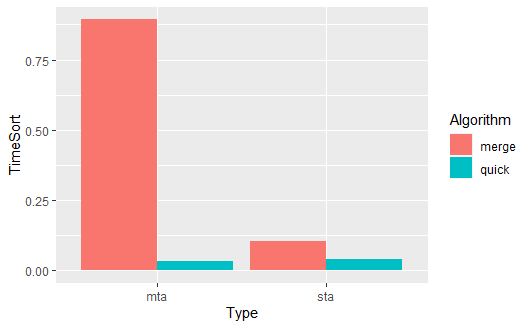
\includegraphics[scale=0.5]{./figures/exp2_comparison_i3_sort.png}
	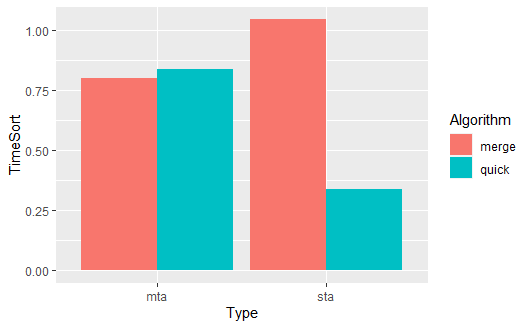
\includegraphics[scale=0.5]{./figures/exp2_comparison_i4_sort.png}
	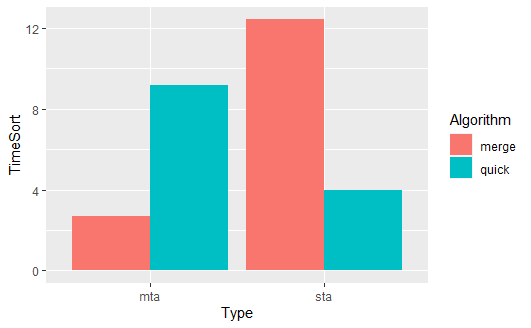
\includegraphics[scale=0.5]{./figures/exp2_comparison_i5_sort.png}
	\centering
	\caption{Comparison of time spent for each sorting algorithm, divided by type for entries i = 3; 4; 5 respectively}
	\label{fig:exp2}
\end{figure}

\section{Discussion and Conclusion}
As presented in the result section, the parallel Merge Sort performed better than the parallel Quick Sort in terms of core usage and time required to complete, as can be seen in figure~\ref{fig:exp1_totalTime}. This observation also translates over to the varying data input sizes, with their most optimal amount of cores $p$ utilized, although this can only be said for inputs of size $10^4$ and above. Below this, the parallel Merge Sort takes more time than the parallel Quick Sort.\\
The trend observed is in contrast to their normal counterparts, where classical Quick Sort remained faster. Of note is one observation, where for i=9, the classical Merge Sort, which was still slower than the classical Quick Sort, was faster than the parallel Quick Sort, as can be seen in figure~\ref{fig:exp2_i9}. Of further note, beginning from i=5, the parallel Merge Sort also became faster than the classical Quick Sort.

\begin{figure}[h]
	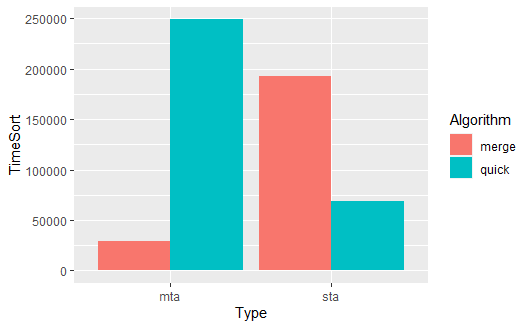
\includegraphics[scale=0.5]{./figures/exp2_comparison_i9_sort.png}
	\centering
	\caption{Comparison of time spent for each sorting algorithm for i=9}
	\label{fig:exp2_i9}
\end{figure}

To conclude this report, we presented 


\end{document}
